\documentclass[12pt,a4paper]{apa}
\usepackage[utf8]{inputenc}
\usepackage{amsmath}
\usepackage{amsfonts}
\usepackage{amssymb}
\usepackage{makeidx}
\usepackage{graphicx}
\usepackage[bahasa]{babel}
\usepackage{apacite}
\threeauthors{Satrio Adityo}{Rizki}{Hamim Tohari}
\threeaffiliations{1103120029}{1103120042}{1103124294\\S1 Teknik Informatika, Universitas Telkom}
\title{\textbf{\textit{Opennes} dan \textit{Heterogeneity}}}
\abstract{Sistem terdistribusi melibatkan interaksi antar perangkat komputer yang otonom atau perangkat yang saling terhubung dan saling koordinasi. Adanya interaksi antar perangkat dalam sistem terdistribusi memunculkan beberapa tantangan dalam pengembangannya. Tantangan dalam sistem terdistribusi diantaranya adalah heterogenitas dan keterbukaan.
\\[0.1cm]	
\emph{\textbf{Keywords :} sistem terdistribusi, tantangan, opennes, heterogeneity}
}
\begin{document}
	\maketitle
	\section{\textbf{Heterogenitas}}
	Keberagaman merupakan karakteristik dari sistem terdistribusi. Keberagaman dalam sistem terdistribusi dapat ditemukan pada jaringan, perangkat keras, sistem operasi, bahasa pemrograman, maupun implementasi oleh pengembang yang berbeda. \cite{Coulouris2012} \cite{Belapurkar2009}
	\subsection{\textbf{Jaringan}}
	Pada jaringan komputer, terdapat beragam protokol jaringan yang dapat digunakan. Dalam satu jaringan lokal dapat terbentuk oleh lebih dari satu protokol jaringan, misal \emph{Ethernet} dan \emph{Wireless Fidelity}. Namun, setiap protokol jaringan memilki standar komunikasi yang konvergen, yaitu \emph{Internet Protocol}. Sehingga, beragam perangkat dapat berkomunikasi tanpa kendala walaupun berbeda protokol jaringannya. \cite{Coulouris2012}
	\subsection{\textbf{Perangkat Keras}}
	Arsitektur yang beragam dapat mempengaruhi mekanisme representasi tipe data perangkat tersebut. Sehingga, program perlu disesuaikan oleh standar tertentu agar mampu saling bertukar data pada perangkat yang beragam. \cite{Coulouris2012}
	\subsection{\textbf{Sistem Operasi}}
	Komputer pada suatu jaringan berkomunikasi dengan \emph{Internet Protocol}. Namun, sistem operasi memiliki metode yang berbeda dalam implementasinya. Misal, Linux / UNIX berbeda metode pertukaran datanya dengan Windows \cite{Coulouris2012}
	\subsection{\textbf{Bahasa Pemrograman}}
	Perbedaan bahasa pemrograman juga menyebabkan perbedaan pada representasi karakter dan struktur data. Jika ingin saling berkomunikasi antarprogram dengan bahasa yang berbeda, diperlukan metode tertentu. Sehingga, walaupun bahasa pemrograman berbeda dalam pengembangannya, namun program dapat saling bertukar data. \cite{Coulouris2012}
	\subsection{\textbf{Pengembangan oleh Banyak Pengembang}}
	Pengembangan program untuk dapat saling berkomunikasi diperlukan standar dan aturan yang seragam. Sehingga, produk yang berbeda dapat saling berkomunikasi dengan program sejenis walaupun memiliki layanan yang berbeda. Pada lingkungan pengembang dan peneliti, standar tersebut dapat ditemukan pada RFC (\emph{Request for Comment}).
	\subsubsection{\textbf{Middleware}}
	\emph{Middleware} merupakan \emph{software layer} yang menyediakan abstraksi untuk mengatasi keberagaman pada sistem terdistribusi. \emph{Middleware} diimplementasikan di atas \emph{Internet Protocol}. \emph{Middleware}, menyediakan model komputasi yang seragam untuk digunakan programmer, sehingga masalah keberagaman dapat diatasi. \cite{Coulouris2012}
	\subsubsection{\textbf{Keberagaman dan Mobile Code}}
	Program dapat berjalan tidak hanya pada \emph{host} pengembang. Pada program \emph{native}, kode program akan dikompilasi menjadi set instruksi yang dikenal oleh arsitektur perangkat tujuan. Namun, pada kasus lain  seperti Java, kode program tidak dikompilasi kedalam set instruksi terendah pada perangkat. Tetapi, kode program akan dikompilasi dalam bentuk set instruksi yang dikenal \emph{Java Virtual Machine}. Kemudian eksekusi program diinterpretasikan oleh \emph{JVM} ketika dijalankan. Contoh lainnya yaitu \emph{javascript}. \cite{Coulouris2012}
	
	Contoh implementasi keberagaman dalam sistem terdistribusi : Intranet, Internet dan mobile computing \cite{Kamalapur2008}
	\subsubsection{\textbf{Intranet}}
		\begin{figure}[h]
		\centering
		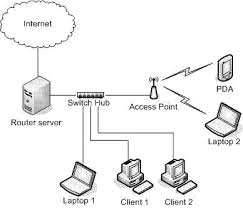
\includegraphics[width=0.5\linewidth]{img/heteroLAN}
		\caption{Heterogenitas pada jaringan lokal, ditunjukkan pada perbedaan protokol jaringan klien.}
		\label{fig:heteroLAN}
		\end{figure}

		Beberapa komputer di suatu ruangan yang terhubung dengan LAN dapat membentuk suatu jaringan kecil. Jika ada beberapa ruangan yang ruangan tersebut saling terhubung, maka terbentuklah jaringan yang lebih besar, yang dapat disebut Intranet.
		
		Jumlah komputer yang terhubung bisa berbeda-beda tiap tempat, tergantung dari pihak yang terlibat dalam pembuatan jaringan. Salah satu contoh penggunaan intranet dalam sistem terdistribusi adalah jaringan lokal suatu universitas.
		
	\subsubsection{\textbf{Internet}}
		
		Internet bisa dikatakan sistem terdistribusi yang sangat besar. Karena setiap perangkat komputer di seluruh dunia dapat terhubung ke dalam satu jaringan yang sama. Dengan adanya Internet ini, komputer dapat digunakan untuk berkomunikasi, bertukar data dengan komputer yang lainya tanpa dibatasi oleh jarak dan waktu. Protokol jaringan dan perangkat yang beragam dapat berkomunikasi dengan adanya konvergensi \emph{Internet Protocol} dan \emph{middleware}.
		
	\subsubsection{\textbf{Mobile Computing}}
		
		Kini, sudah banyak \emph{device} yang dilengkapi dengan jaringan nirkabel yang memungkinkan pengguna dapat terhubung ke jaringan lokal. \emph{Mobile computing} dapat diartikan sebagai perangkat lunak atau perangkat keras yang terhubung ke jaringan, sehingga dapat digunakan saat terhubung ke jaringan melalui jaringan nirkabel.
		
		Akibat adanya keberagaman ini, ada permasalahan yang timbul ketika tiap perangkat harus saling berkomunikasi. Dengan pengembangan yang berbeda dan perangkat keras yang berbeda akan terjadi kesulitan dalam komunikasi dan pertukaran data.
		
		\begin{figure}[h]
		\centering
		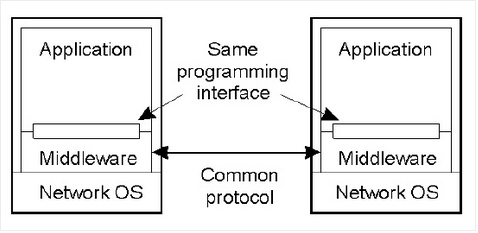
\includegraphics[width=0.5\linewidth]{img/middleware}
		\caption{Sistem terdistribusi dengan \emph{middleware} sebagai \emph{interfaces} antaraplikasi}
		\label{fig:middleware}
		\end{figure}

		
		Untuk mengatasi masalah tersebut, diperlukan adanya \emph{middleware}. Dengan adanya \emph{middleware} perangkat yang dibangun dalam jaringan, hardware, sistem operasi, dan bahasa pemrograman yang berbeda bisa saling berkomunikasi karena mampu memberikan abstraksi yang memungkinkan semua aplikasi berbeda berjalan di atasnya dengan standar yang ditentukan. \cite{Coulouris2012}
	%------------------------------------------------------
	\section{\textbf{Keterbukaan}}
	\begin{figure}[h]
	\centering
	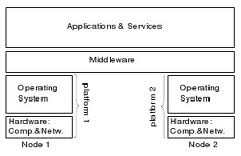
\includegraphics[width=0.5\linewidth]{img/openness}
	\caption{Dengan \emph{openness} pada sistem terdistribusi, layanan dapat ditambahkan tanpa mengganggu komponen lain.}
	\label{fig:openness}
	\end{figure}

	Selain keberagaman, tantangan lain dalam pengembangan sistem terdistribusi adalah bagaimana membuat sistem dapat terus dikembangkan dan tetap berjalan sebagaimana mestinya. Hal inilah yang dimaksud dengan keterbukaan (\emph{openness}) \cite{Coulouris2012}. Sistem harus mampu dikembangkan dan ditambahkan berbagai layanan. Sehingga, antarlayanan dapat saling berbagi \emph{resources}, tersinkron, dan terhubung. \cite{Coulouris2012}
	
	Ciri utama dari sistem yang mendukung keterbukaan adalah dokumentasi dan spesifikasinya yang dipublikasikan secara umum \cite{Kamalapur2008}. Publikasi ini memungkinkan semua pengembang untuk  mengembangakan sistem tersebut bersama-sama dan tetap mengacu pada standar yang telah disepakati bersama.
	
	Namun ada masalah baru yang mungkin muncul dari publikasi ini. Seperti yang dijelaskan pada isu \emph{heterogeneity}, setiap pengembang memiliki karakteristik yang berbeda-beda dalam melakukan pengembangan sistem. Jika hal ini tidak ditangani, maka sistem tidak akan bisa berjalan sebagaimana mestinya. Oleh karena itu, diperlukan sebuah aturan dan sintaks baku yang harus digunakan dalam pengembangan sistem \cite{Tanenbaum2007}. Misalnya saja pada jaringan komputer, terdapat dokumen yang dikenal dengan RFC. Dengan spesifikasi dan standar yang jelas sehingga pengembang diharapkan mengacu pada dokumen tersebut.
	
	Selain jaringan, \emph{openness} dalam sistem terdistribusi juga bisa lihat dari pengembangan www atau yang sering dikenal dengan nama situs web. www ini dikembangkan oleh W3C (World Wide Web Consortium). Organisasi yang dibuat oleh Tim Barners-Lee pada tanggal 20 Oktober 1994 di MIT ini mengajak semua orang untuk mengembangkan standar-standar untuk www. Salah satu standarisasinya adalah tentang bahasa \emph{scripting} untuk desain web seperti HTML, XML, dan lain- lain. Dengan adanya dokumentasi standar yang dibuat ini, maka pengembang yang ingin melakukan pengembangan harus mengikuti standar tersebut. 
	
	Keharusan sistem terdistribusi untuk memiliki karakteristik \emph{openness} menimbulkan tantangan baru, yaitu kompleksitas sistem yang bisa jadi semakin rumit \cite{Coulouris2012}. Olehkarenanya diperlukan suatu penanganan khusus untuk menangani hal ini. Selain itu, setiap perangkat atau standar yang ditambahkan ke sistem terdistribusi yang sudah ada harus dilakukan pengecekan apakah bisa berjalan dengan baik atau tidak. \cite{Coulouris2012}
	
	\bibliographystyle{apacite}
	\bibliography{laporanreferensi}
	\newpage
	
	\begin{center}
		\textbf{Kontribusi}
	\end{center}
	\begin{description}
		\item[Satrio] 35\%
		\item[Rizki] 30\%
		\item[Hamim] 35\%
	\end{description}
\end{document}